\documentclass[11pt,a4paper]{article}
\usepackage{iftex}
\ifPDFTeX
  \usepackage[T1]{fontenc}
\fi
\usepackage[turkish,shorthands=:!]{babel}
\usepackage[margin=2.5cm]{geometry}
\usepackage{amsmath,amssymb}
\usepackage{graphicx}
\usepackage{booktabs}
\usepackage{caption}
\usepackage{tikz}
\usetikzlibrary{babel}
\usepackage{pgfplots}
\pgfplotsset{compat=1.18}
\usepackage[hidelinks]{hyperref}

\title{Makale Başlığı}
\author{Yazar Bir\thanks{Kurum, e-posta} \and Yazar İki}
\date{\today}

\begin{document}
\maketitle

\begin{abstract}
Bu çalışmada \ldots{} incelenmiştir. Önerilen yöntem, karşılaştırılan
yöntemlere göre daha yüksek doğruluk sağlamaktadır.
\end{abstract}

\section{Giriş}
Konunun arka planı ve literatür \cite{knuth1984}. Çalışmanın katkıları
Bölüm~\ref{sec:yontem} ve Bölüm~\ref{sec:bulgular}'da sunulmaktadır.

\section{Yöntem}\label{sec:yontem}
Model aşağıdaki denklemle tanımlanır:
\begin{equation}\label{eq:model}
  y = \beta_0 + \beta_1 x + \varepsilon, \qquad \varepsilon \sim \mathcal{N}(0,\sigma^2).
\end{equation}

\section{Bulgular}\label{sec:bulgular}
Denklem~\eqref{eq:model} ile elde edilen sonuçlar Şekil~\ref{fig:sonuc}
ve Tablo~\ref{tab:sonuc}'da verilmiştir.

\begin{figure}[ht]
  \centering
  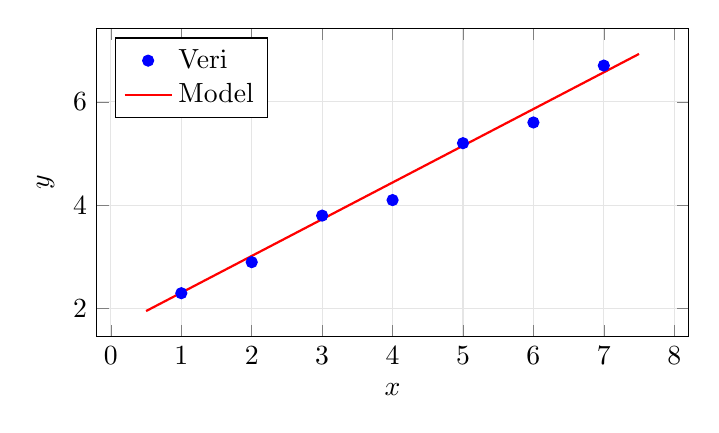
\begin{tikzpicture}
  \begin{axis}[
    width=0.75\linewidth, height=5.5cm,
    xlabel={$x$}, ylabel={$y$},
    grid=major, grid style={gray!20},
    legend pos=north west, legend cell align=left,
  ]
    \addplot[only marks, mark=*, blue] coordinates {
      (1,2.3) (2,2.9) (3,3.8) (4,4.1) (5,5.2) (6,5.6) (7,6.7)
    };
    \addlegendentry{Veri}
    \addplot[thick, red, domain=0.5:7.5] {1.6 + 0.71*x};
    \addlegendentry{Model}
  \end{axis}
\end{tikzpicture}
  \caption{Ölçülen değerler ve model.}
  \label{fig:sonuc}
\end{figure}

\begin{table}[ht]
  \centering
  \caption{Yöntemlerin karşılaştırılması.}
  \label{tab:sonuc}
  \begin{tabular}{lcc}
    \toprule
    Yöntem & Doğruluk (\%) & Süre (s) \\
    \midrule
    Yöntem 1 & 81{,}2 & 12{,}4 \\
    Yöntem 2 & 84{,}7 & 15{,}1 \\
    Önerilen & \textbf{90{,}3} & 13{,}0 \\
    \bottomrule
  \end{tabular}
\end{table}

\section{Sonuç}
Elde edilen bulgular \ldots{} göstermektedir.

\begin{thebibliography}{9}
  \bibitem{knuth1984} D.~E. Knuth, \emph{The \TeX book}, Addison-Wesley, 1984.
  \bibitem{tantau} T.~Tantau, \emph{The TikZ and PGF Packages}, 2023.
\end{thebibliography}

\end{document}
